%!TEX root = ../thesis.tex

\section{実験概要}
%\begin{figure}[hbtp]
  %\centering
 %\includegraphics[keepaspectratio, scale=0.8]
      %{images/RaspberryPiMouse.png}
 %\caption{Example}
 %\label{Fig:Example}
%\end{figure}
%\subsection{実験概要}
本研究では,本研究室で開発されているロボット ORNE-box3\cite{井口颯人2023屋外自律移動ロボットプラットフォーム-orne} を用いて走行実験を行った.実機ロボットの外観は\figref{Fig:ORNE-box3}に示す.ORNE-box3のセンサ構成については、\figref{Fig:sensor configuration}に示すように,PCとしてJetson Orin NX 16GBを搭載しており、3D LiDAR:R-Fans-16
、IMU:ADIS16465、Encoder : i-Cart middleを備えている.3D LiDARは、自己位置推定と障害物検知に使用し、IMUとエンコーダは、emcl2に対して情報を提供している.

走行ルートは\figref{Fig:Course map of the Tsudanuma Challenge 2025}が示すように,津田沼校舎2号館前から食堂前に設置されたコーンまでとし,
津田沼チャレンジのコースの一部を利用した.このルートは,屋外環境における
自律移動性能を評価するための実環境を想定したものである.


実験では,Navigation2 における各種パラメータを個別に変化させた場合の
ロボットの挙動の変化を調査することを目的とした.
各走行実験においては,対象とするパラメータのみを変更し,
それ以外のパラメータはすべて一定に保った.

また,パラメータの変更に際しては,変更前の設定値を基準値とし,
基準値から増減させた場合のロボットの走行挙動を比較・分析した.
これにより,各パラメータがロボットの走行安定性や挙動に与える影響を
明確にすることを試みた.

\begin{figure}[hbtp]
  \centering
 \includegraphics[keepaspectratio, scale=0.6]
      {images/tsudanumachallenge.png}
 \caption{Course map of the Tsudanuma Challenge 2025(source: \cite{Tsudanumachallenge})}
 \label{Fig:Course map of the Tsudanuma Challenge 2025}
\end{figure}

\begin{figure}[hbtp]
  \centering
 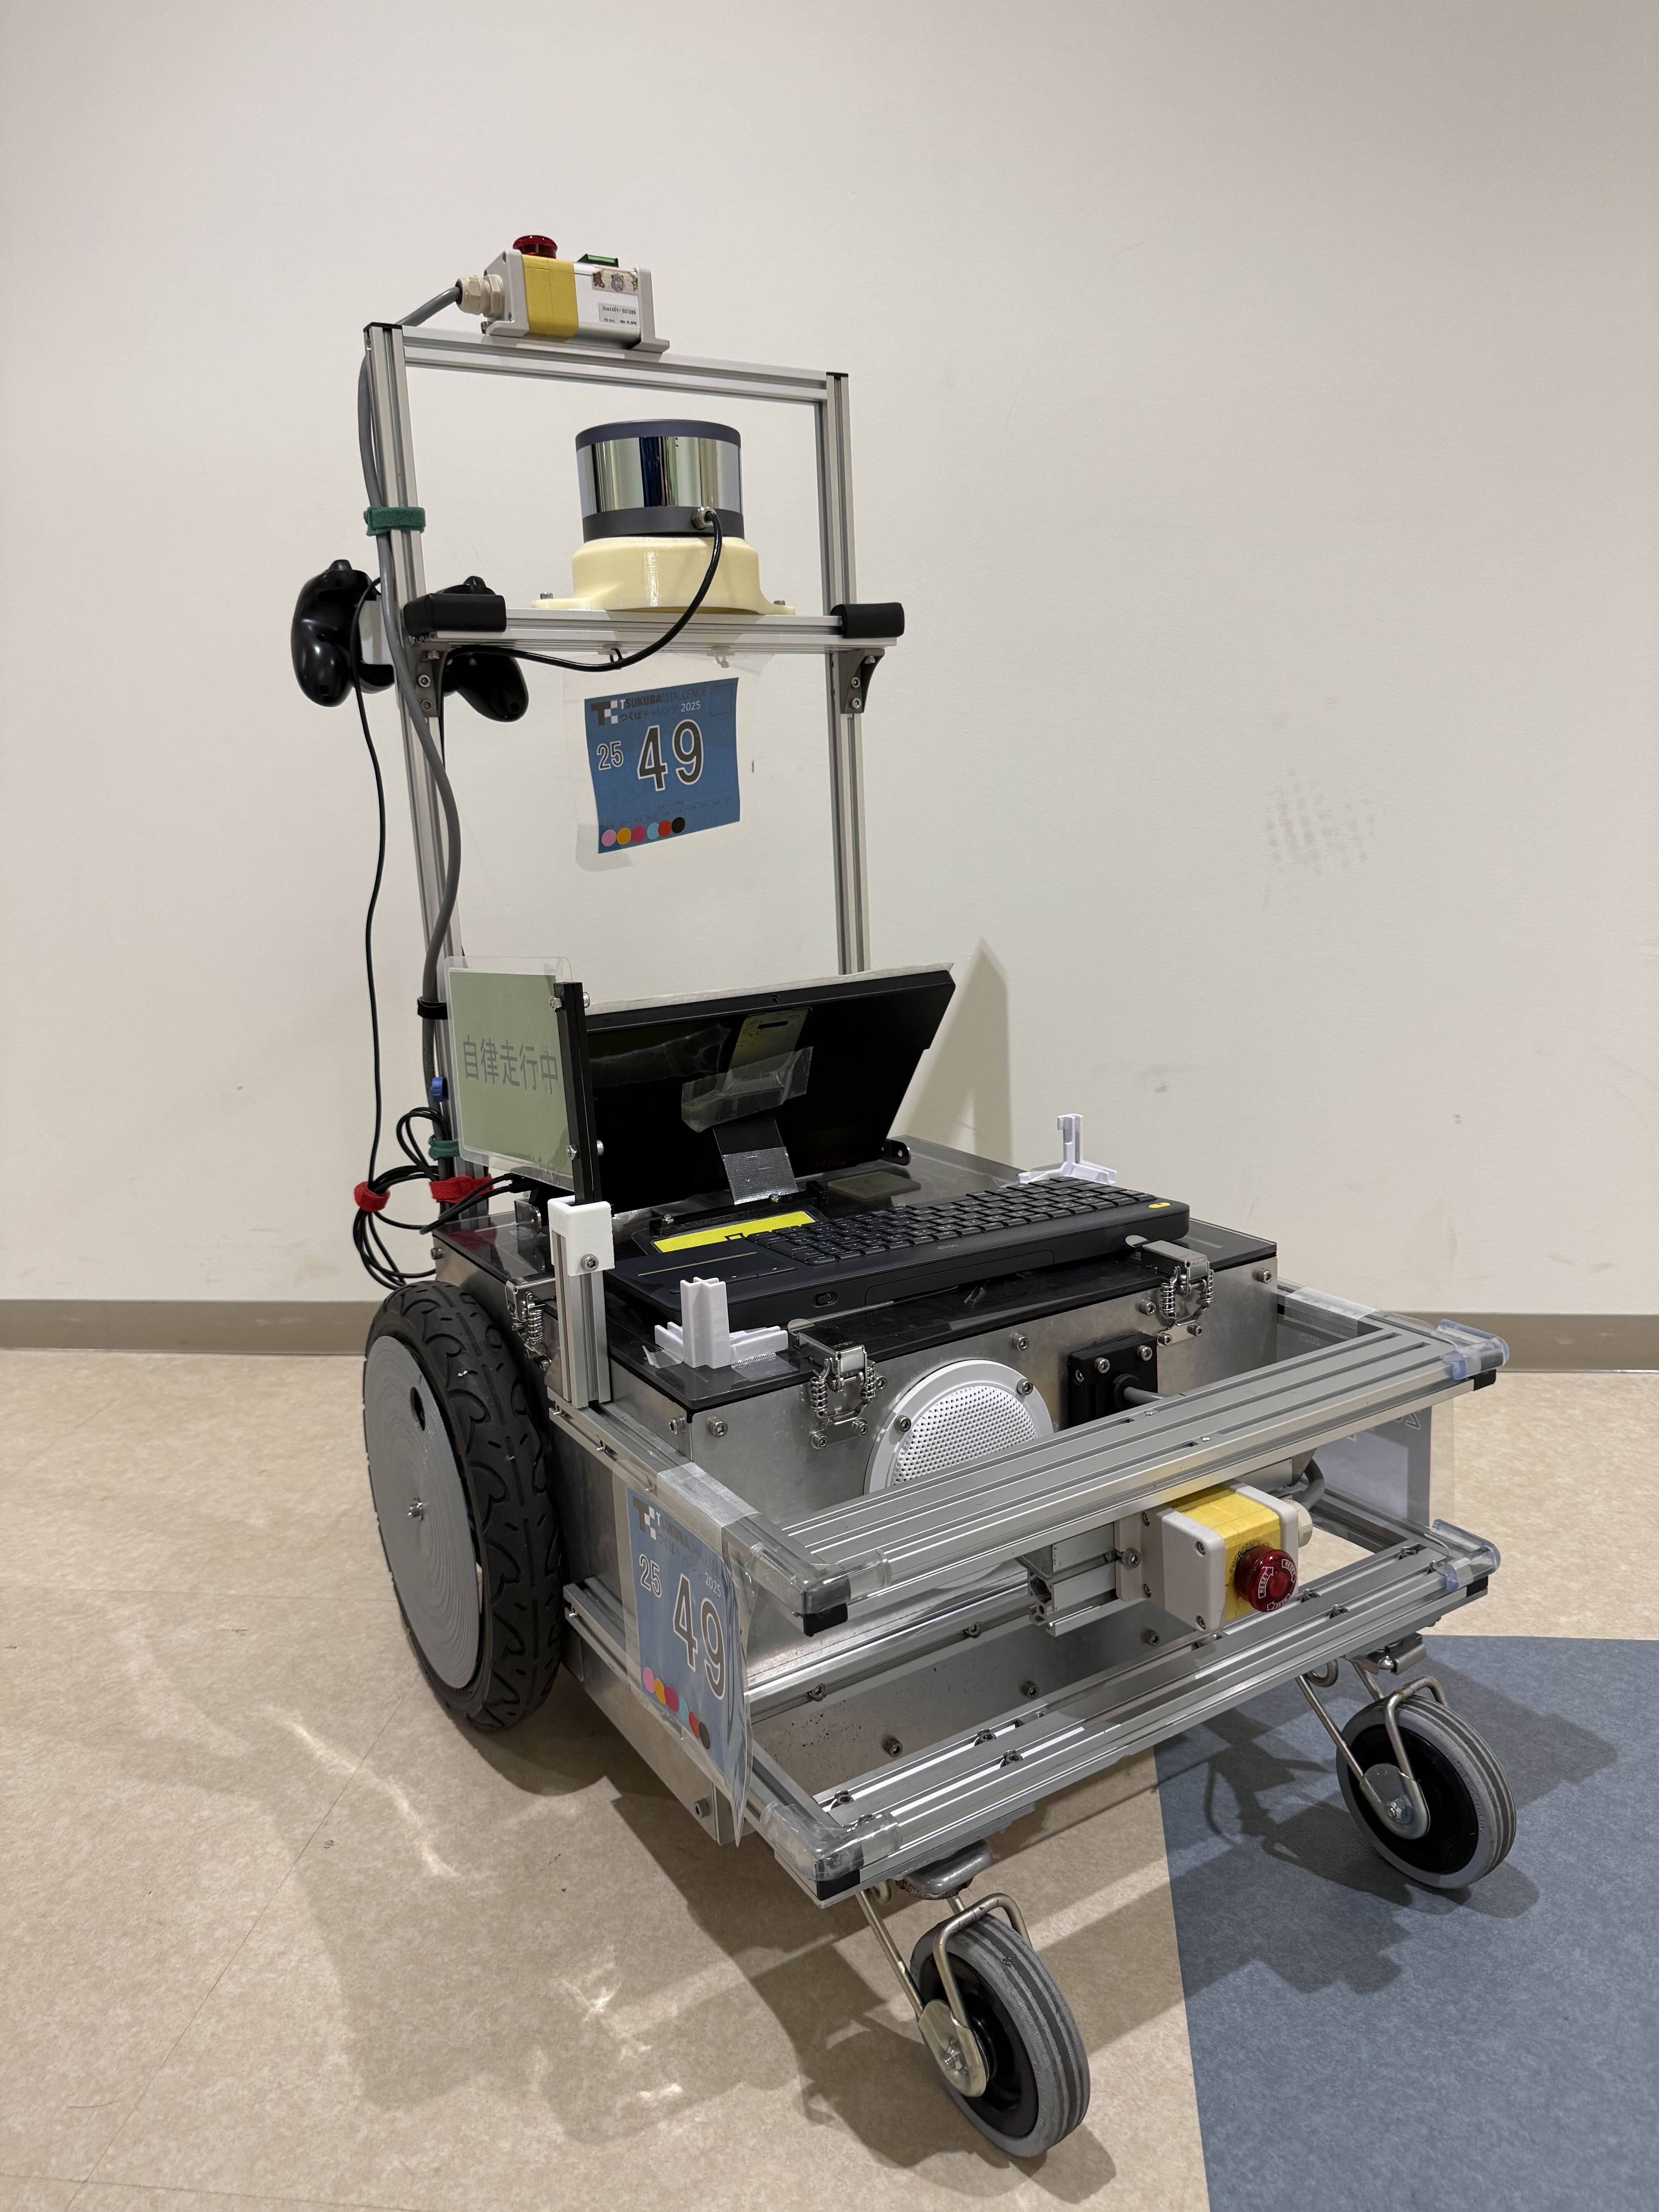
\includegraphics[keepaspectratio, scale=0.3]
      {images/orne-box3.png}
 \caption{ORNE-box3(source: \cite{井口颯人2023屋外自律移動ロボットプラットフォーム-orne})}
 \label{Fig:ORNE-box3}
\end{figure}
\begin{figure}[hbtp]
  \centering
 \includegraphics[keepaspectratio, scale=0.3]
      {images/sensor.png}
 \caption{sensor configuration}
 \label{Fig:sensor configuration}
\end{figure}
%\subsubsection{etc...}






\newpage

\section{実験結果}
%\begin{figure}[hbtp]
  %\centering
 %\includegraphics[keepaspectratio, scale=0.8]
      %{images/RaspberryPiMouse.png}
 %\caption{Example}
 %\label{Fig:Example}
%\end{figure}
\subsection{実験結果(emcl2)}
\subsubsection{実験結果(num\_particles)}
\begin{table}[H]
  \centering
  \caption{パーティクル数の違いによるゴール到達可否}
  \label{tab:num_particles_result}
  \begin{tabular}{c|c|c|c}
    \hline
    number of times & 200 & 500 (base) & 1000 \\
    \hline
    1  & $\times$ & ○ & ○ \\
    2  & ○ & ○ & $\times$ \\
    3  & $\times$ & $\times$ & $\times$ \\
    4  & ○ & ○ & ○ \\
    5  & ○ & ○ & $\times$ \\
    6  & $\times$ & $\times$ & $\times$ \\
    7  & ○ & ○ & ○ \\
    8  & ○ & ○ & ○ \\
    9  & ○ & ○ & ○ \\
    10 & ○ & ○ & ○ \\
    \hline
  \end{tabular}
\end{table}


\subsubsection{実験結果(odom\_fw\_dev\_per\_fw)}


\subsection{実験結果(Nav2\_controller)}

\subsection{実験結果(Nav2\_Costmap)}

\subsection{実験結果(Nav2\_Velocity Smoother)}

\subsection{実験結果(Nav2\_planner goal)}


%\subsubsection{etc...}